\section{The cross product}

\begin{outcome}
\begin{enumerate}
\item[A.] Compute the cross product of vectors algebraically and
  geometrically.
\item[B.] Compute the box product of three vectors in $\R^3$. 
\item[C.] Determine whether a system of three vectors in $\R^3$ is
  right-handed, algebraically and geometrically.
\item[D.] Find the area of a parallelogram determined by two vectors
  in $\R^3$.
\item[E.] Find the area of a triangle determined by three points in
  $\R^3$.
\item[F.] Find the volume of a parallelepiped determined by three
  vectors in $\R^3$.
\item[G.] Use properties of the cross product and the dot product to
  prove algebraic equalities.
\end{enumerate}
\end{outcome}

Unlike the dot product, the cross product is only defined in $\R^3$,
i.e., only in 3-dimensional space. The cross product of two vectors is
a vector.

We will first discuss the geometric meaning of the cross product, and
then give an algebraic description. Both descriptions are equally
important: the geometric description is essential for applications in
physics and geometry, whereas the algebraic description is necessary
for computing.

% ----------------------------------------------------------------------
\subsection{Right-handed systems of vectors}

We begin with a discussion of right-handed systems of vectors in
3-dimensional
space.\index{right handed system of vectors}\index{vector!right-handed system of}

\begin{definition}{Right-handed system of vectors}{righthand}
  Three vectors, $\vect{u},\vect{v},\vect{w}$ form a right-handed
  system if when you extend the thumb of your right hand in the
  direction of $\vect{u}$ and your index finger in the direction of
  $\vect{v}$, your relaxed middle finger points roughly in the
  direction of $\vect{w}$.
  \begin{center}
    \raisebox{0.25in}{
      \begin{tikzpicture}
        \draw[->](0,0,0) -- node[right] {$\vect{u}$} (0,2,0);
        \draw[->](0,0,0) -- node[above] {$\vect{v}$} (-2,0,0);
        \draw[->](0,0,0) -- node[right] {$\vect{w}$} (0,0,3);
      \end{tikzpicture}
    }
    \hspace{1in}
    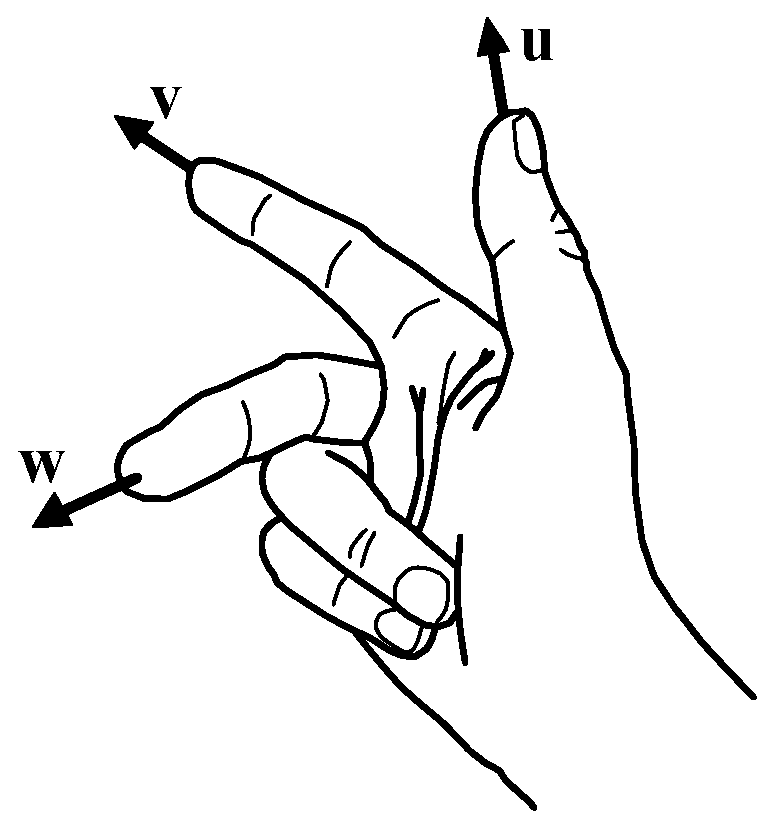
\includegraphics[height=2in]{figures/right-handed}
  \end{center}
\end{definition}

You should consider how a right-handed system would differ from a
left-handed system. Try using your left hand and you will see that the
vector $\vect{w}$ would need to point in the opposite direction.

Recall the special vectors $\vect{i}=\mat{1,0,0}^T$,
$\vect{j}=\mat{0,1,0}^T$, and $\vect{k}=\mat{0,0,1}^T$ we saw in
Section~\ref{sec:linear-combinations-rn}. We always assume that our
coordinate system is drawn in such a way that the vectors $\vect{i}$,
$\vect{j}$, $\vect{k}$ form a right-handed system. Thus, if the thumb
of your right hand points along the $x$-axis and your index finger
points along the $y$-axis, your middle finger should point along the
$z$-axis. 

\begin{center}
\begin{tikzpicture}
\draw[->, thick] (0,0,0)--(2,0,0);
\draw[->, thick] (0,0,0)--(0,2,0);
\draw[->, thick] (0,0,0)--(0,0,2);
\node[below right] at (2,0,0){$\vect{j}$};
\node[below left] at (0,0,2){$\vect{i}$};
\node[above right] at (0,2,0){$\vect{k}$};
\end{tikzpicture}
\end{center}

% ----------------------------------------------------------------------
\subsection{Geometric description of the cross product}

The following is the geometric description of the cross
product. Recall that the dot product of two vectors results in a
scalar. In contrast, the cross product results in a vector, as the
cross product gives a direction as well as
a magnitude.\index{cross product!geometric description}

\begin{definition}{Geometric definition of cross product}{crossprodgeomet}
  Let\/ $\vect{u}$ and $\vect{v}$ be two vectors in $\R^{3}.$ Their
  \textbf{cross product}\index{cross product}, written
  $\vect{u}\times \vect{v}$, is the vector defined by the following three rules.
  \index{cross product!geometric description}

\begin{enumerate}
\item Its length is $\norm{\vect{u}\times \vect{v}} =\norm{\vect{u}} \norm{
\vect{v}} \sin \theta $, 
where $\theta $ is the included angle between $\vect{u}$ and $\vect{v}$.

\item It is orthogonal to both $\vect{u}$ and $\vect{v}$.

\item The vectors $\vect{u}$, $\vect{v}$, and $\vect{u}\times
  \vect{v}$, in that order, form a right-handed system.
\end{enumerate}
\end{definition}

We note that the length of the cross product,
$\norm{\vect{u}\times\vect{v}}$, given by the formula
$\norm{\vect{u}}\norm{\vect{v}}\sin\theta$, is the area of the
parallelogram determined by $\vect{u}$ and $\vect{v}$, as shown in the
following picture.\index{cross product!area of parallelogram}
\begin{center}
  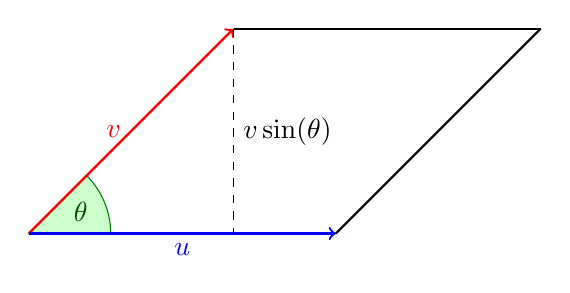
\begin{tikzpicture}[scale=1.3]
    \filldraw[fill=green!20,draw=green!50!black] (0,0) -- (0:8mm) arc (0:45:8mm) -- cycle;
    \draw[->,thick,red] (0,0) -- node[left] {$\vect{v}$} (2,2);
    \draw[->,thick,blue] (0,0) -- node[below] {$\vect{u}$} (3,0);
    \draw[thick] (2,2)--(5,2);
    \draw[thick] (3,0)--(5,2);
    \draw[dashed] (2,2)--(2,0);
    \node[green!30!black] at (22.5:5.5mm) {$\theta$};
    \node[right] at (2,1){$\norm{\vect{v}} \sin(\theta)$};
  \end{tikzpicture}
\end{center}

% ----------------------------------------------------------------------
\subsection{Algebraic definition of the cross product}

From its geometric description, we can prove that the cross product
satisfies the following properties.

\begin{proposition}{Properties of the cross product}{propertiescrossproduct}
  Let $\vect{u}, \vect{v}, \vect{w}$ be vectors in $\R^3$, and $k$ a
  scalar. Then the following hold.
  \begin{enumerate}
  \item
    $\vect{u}\times \vect{v}= -\tup{\vect{v}\times \vect{u}}$,
    and $\vect{u}\times \vect{u}=\vect{0}$.
  \item $\tup{k \vect{u}}\times \vect{v}= k \tup{\vect{u}\times \vect{v}} 
    =\vect{u}\times \tup{k \vect{v}}$.
  \item $\vect{u}\times \tup{\vect{v}+\vect{w}} =\vect{u}\times \vect{v}+\vect{u}\times \vect{w}$.
  \item $\tup{\vect{v}+\vect{w}} \times \vect{u}=\vect{v} \times \vect{u}+\vect{w}\times \vect{u}$.
  \end{enumerate}
\end{proposition}

\begin{proof}
  Formula $1.$ follows immediately from the definition. The vectors
  $\vect{u}\times \vect{v}$ and $\vect{v}\times \vect{u}$ have the
  same magnitude, $\norm{\vect{u}}\norm{\vect{v}}\sin \theta ,$ and an
  application of the right hand rule shows they have opposite
  direction.

  Formula $2.$ is proven as follows. If $k $ is a non-negative scalar,
  the direction of $\tup{k \vect{u}} \times \vect{v}$ is the same as
  the direction of
  $\vect{u}\times \vect{v}, k \tup{\vect{u}\times \vect{v}} $ and
  $\vect{u}\times \tup{ k \vect{v}} $. The magnitude is $k$ times the
  magnitude of $\vect{u}\times \vect{v}$ which is the same as the
  magnitude of $k \tup{\vect{u}\times \vect{v}} $ and
  $\vect{u}\times \tup{ k \vect{v}} .$ Using this yields equality in
  $2$. In the case where $k <0,$ everything works the same way except
  the vectors are all pointing in the opposite direction and you must
  multiply by $\abs{k }$ when comparing their magnitudes.

  The distributive laws, $3.$ and $4.$, are harder to establish. For
  now, we will content ourselves with noticing that if we know that
  $3.$ is true, $4.$ follows. Namely, assuming $3.$, and using $1.$,
  we have
  \begin{align*}
    \tup{\vect{v}+\vect{w}} \times \vect{u}
    & =-\vect{u}\times \tup{
      \vect{v}+\vect{w}} \\
    & =-\tup{\vect{u}\times \vect{v}+\vect{u}\times \vect{w}} \\
    & =\vect{v}\times \vect{u}+\vect{w}\times \vect{u}.
  \end{align*}
\end{proof}

In turn, we can use the properties from
Proposition~\ref{prop:propertiescrossproduct} to get an algebraic
description of the cross product. We begin by determining the cross
products of the special vectors $\vect{i}$, $\vect{j}$, and
$\vect{k}$. They are as follows:
\begin{equation*}
  \begin{array}{c@{\quad\quad}c@{\quad\quad}c}
    \vect{i}\times \vect{j}=\vect{k},
    & \vect{j}\times \vect{i}=-\vect{k},
    & \vect{i}\times \vect{i}=\vect{0}, \\
    \vect{k}\times \vect{i}=\vect{j},
    & \vect{i}\times \vect{k}=-\vect{j},
    & \vect{j}\times \vect{j}=\vect{0}, \\
    \vect{j}\times \vect{k}=\vect{i},
    & \vect{k}\times \vect{j}=-\vect{i},
    & \vect{k}\times \vect{k}=\vect{0}.
  \end{array}
\end{equation*}
With this information and the laws of
Proposition~\ref{prop:propertiescrossproduct}, we can compute the cross
product of any two vectors from their coordinates.\index{cross product!coordinate description}
Let
\begin{equation*}
  \vect{u}=\begin{mymatrix}{c}u_1\\u_2\\u_3\end{mymatrix}
  \quad\mbox{and}\quad
  \vect{v}=\begin{mymatrix}{c}v_1\\v_2\\v_3\end{mymatrix}.
\end{equation*}
Then we have:
\begin{eqnarray*}
  \vect{u}\times\vect{v}
  &=& (u_{1}\vect{i}+u_{2}\vect{j}+u_{3}\vect{k})\times (v_{1}\vect{i}+v_{2}\vect{j}+v_{3}\vect{k})\\
  &=& \begin{array}[t]{@{}c@{~}c@{~}c@{~}c@{~}c@{~}c}
          & u_1v_1(\vect{i}\times\vect{i})
        &+& u_1v_2(\vect{i}\times\vect{j})
        &+& u_1v_3(\vect{i}\times\vect{k})\\
         +& u_2v_1(\vect{j}\times\vect{i})
        &+& u_2v_2(\vect{j}\times\vect{j})
        &+& u_2v_3(\vect{j}\times\vect{k})\\
         +& u_3v_1(\vect{k}\times\vect{i})
        &+& u_3v_2(\vect{k}\times\vect{j})
        &+& u_3v_3(\vect{k}\times\vect{k})
      \end{array}
  \\
  &=&\begin{array}[t]{@{}c@{~}c@{~}c@{~}c@{~}c@{~}c}
         & u_1v_1\vect{0}
       &+& u_1v_2\vect{k}
       &-& u_1v_3\vect{j}\\
        -& u_2v_1\vect{k}
       &+& u_2v_2\vect{0}
       &+& u_2v_3\vect{i}\\
        +& u_3v_1\vect{j}
       &-& u_3v_2\vect{i}
       &+& u_3v_3\vect{0}
     \end{array}
  \\
  &=& (u_{2}v_{3}-u_{3}v_{2}) \vect{i}+
      (u_{3}v_{1} - u_{1}v_{3}) \vect{j}+
      (u_{1}v_{2}-u_{2}v_{1}) \vect{k}.
\end{eqnarray*}
The resulting formula for the cross product is summarized in the
following Proposition.

\begin{proposition}{Coordinate description of cross product}{crossprodcoord}
  The cross product can be computed as follows:
  \begin{equation*}
    \begin{mymatrix}{c}u_1\\u_2\\u_3\end{mymatrix}
    \times
    \begin{mymatrix}{c}v_1\\v_2\\v_3\end{mymatrix}
    =
    \begin{mymatrix}{c}
      u_2v_3 - u_3v_2 \\
      u_3v_1 - u_1v_3 \\
      u_1v_2 - u_2v_1 \\
    \end{mymatrix}.
  \end{equation*}
\end{proposition}

\begin{comment}
There is another version of \ref{crossprod1} which may be easier to remember.
We can express the cross product as the determinant of a matrix, as follows. 
\begin{equation}
\vect{u}\times \vect{v} = \begin{absmatrix}{ccc}
\vect{i} & \vect{j} & \vect{k} \\
u_{1} & u_{2} & u_{3} \\
v_{1} & v_{2} & v_{3}
\end{absmatrix} \label{crossprod3}
\end{equation}
Expanding the determinant along the top row yields
\begin{equation*}
\vect{i}\tup{-1} ^{1+1}\begin{absmatrix}{cc}
u_{2} & u_{3} \\
v_{2} & v_{3}
\end{absmatrix}+\vect{j}\tup{-1} ^{2+1}\begin{absmatrix}{cc}
u_{1} & u_{3} \\
v_{1} & v_{3}
\end{absmatrix}+\vect{k}\tup{-1} ^{3+1}\begin{absmatrix}{cc}
u_{1} & u_{2} \\
v_{1} & v_{2}
\end{absmatrix}\end{equation*}
\begin{equation*}
=\vect{i}\begin{absmatrix}{cc}
u_{2} & u_{3} \\
v_{2} & v_{3}
\end{absmatrix}-\vect{j}\begin{absmatrix}{cc}
u_{1} & u_{3} \\
v_{1} & v_{3}
\end{absmatrix}+\vect{k}\begin{absmatrix}{cc}
u_{1} & u_{2} \\
v_{1} & v_{2}
\end{absmatrix}\end{equation*}
Expanding these determinants leads to 
\begin{equation*}
\tup{u_{2}v_{3}-u_{3}v_{2}} \vect{i}-\tup{
u_{1}v_{3}-u_{3}v_{1}} \vect{j}+\tup{u_{1}v_{2}-u_{2}v_{1}}
\vect{k}  
%\label{crossprod4}
\end{equation*}
which is the same as \ref{crossprod2}.
\end{comment}

We will now look at an example of how to compute a cross product.

\begin{example}{Find a cross product}{findcrossproduct}
Find $\vect{u} \times \vect{v}$ for the vectors
\begin{equation*}
\vect{u}
=
\begin{mymatrix}{r}
1 \\
-1 \\
2
\end{mymatrix}
\quad\mbox{and}\quad
\vect{v}
=
\begin{mymatrix}{r}
3 \\
-2 \\
1
\end{mymatrix}.
\end{equation*}
\end{example}

\begin{solution}
  Using Proposition~\ref{prop:crossprodcoord}, we compute
  \begin{equation*}
    \begin{mymatrix}{c}1\\-1\\2\end{mymatrix}
    \times
    \begin{mymatrix}{c}3\\-2\\1\end{mymatrix}
    =
    \begin{mymatrix}{c}
      (-1)(1) - (2)(-2) \\
      (2)(3) - (1)(1) \\
      (1)(-2) - (-1)(3) \\
    \end{mymatrix}
    =
    \begin{mymatrix}{c}
      3 \\
      5 \\
      1
    \end{mymatrix}.
  \end{equation*}
\end{solution}

We use this concept in the following example.

\begin{example}{Area of a parallelogram}{areaparallelogram}
  Find the area of the parallelogram determined by the following
  vectors $\vect{u}$ and $\vect{v}$:
  \begin{equation*}
    \vect{u}
    =
    \begin{mymatrix}{r}
      1 \\
      -1 \\
      2
    \end{mymatrix}, \quad
    \vect{v}
    =
    \begin{mymatrix}{r}
      3 \\
      -2 \\
      1
    \end{mymatrix}.
  \end{equation*}
\end{example}

\begin{solution}
  Notice that these vectors are the same as the ones given in Example
  \ref{exa:findcrossproduct}.  Recall from the geometric description
  of the cross product that the area of the parallelogram is the
  magnitude of $\vect{u} \times \vect{v}$.  From
  Example~\ref{exa:findcrossproduct},
  $\vect{u} \times \vect{v} = \mat{3,5,1}^T$.  
  Thus the area of the parallelogram is 
  \begin{equation*}
    \norm{\vect{u} \times \vect{v}} = 
    \sqrt{3^2+5^2+1^2} = \sqrt{35}.
  \end{equation*}
\end{solution}

We can also use this concept to find the area of a triangle, as in the
following example.

\begin{example}{Area of triangle}{areatriangle}
  Find the area of the triangle determined by the points
  $\tup{1,2,3}$, $\tup{0,2,5}$, and $\tup{5,1,2}$.
\end{example}

\begin{solution}
  Let $P=\tup{1,2,3}$, $Q=\tup{0,2,5}$, and $R=\tup{5,1,2}$. The area
  of the triangle is exactly half of the area of the parallelogram
  determined by the vectors $\longvect{PQ}$ and $\longvect{PR}$.
  \begin{center}
    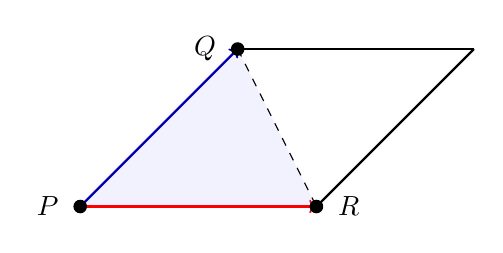
\begin{tikzpicture}[scale=1]
      \fill[blue!5] (0,0) -- (2,2) -- (3,0) -- cycle;
      \draw[->,thick,blue!70!black] (0,0) -- (2,2);
      \draw[->,thick,red] (0,0) -- (3,0);
      \draw[thick] (2,2)--(5,2);
      \draw[thick] (3,0)--(5,2);
      \draw[dashed] (2,2)--(3,0);
      \draw[fill](0,0) circle [radius=2.25pt] node[left=1ex]{$P$};
      \draw[fill](2,2) circle [radius=2.25pt] node[left=1ex]{$Q$};
      \draw[fill](3,0) circle [radius=2.25pt] node[right=1ex]{$R$};
    \end{tikzpicture}
  \end{center}
  We have $\longvect{PQ}=\mat{-1,0,2}^T$ and
  $\longvect{PR}=\mat{4,-1,-1}^T$. The area of the parallelogram is
  the magnitude of the cross product:
  \begin{equation*}
    \norm{\longvect{PQ}\times\longvect{PR}}
    =
    \norm{\begin{mymatrix}{r}
        -1 \\
        0 \\
        2
      \end{mymatrix} \times \begin{mymatrix}{r}
        4 \\
        -1 \\
        -1
      \end{mymatrix}
    }
    = \norm{\begin{mymatrix}{rrr}
        2 \\ 7 \\ 1
      \end{mymatrix}
    }
    = \sqrt{2^2+7^2+1^2}
    = \sqrt{54}.
  \end{equation*}
  Hence the area of the triangle is $\frac{1}{2}\sqrt{54}= \frac{3}{2}\sqrt{6}.$
\end{solution}

In general, the area of the triangle determined by three points
$P,Q,R$ in $\R^3$ is given by
\begin{equation*}
\frac{1}{2}\norm{\longvect{PQ} \times  \longvect{PR}}.
\end{equation*}
